\documentclass[tikz,border=10pt]{standalone}
\usepackage{amsmath}
\usetikzlibrary{arrows.meta, positioning, calc, fit, decorations.pathreplacing}

\definecolor{c1}{HTML}{000000}
\definecolor{c2}{HTML}{233D4D}
\definecolor{c3}{HTML}{FE7F2D}
\definecolor{c4}{HTML}{EAECF0}
\definecolor{labelcolor}{HTML}{5F6B75}

\begin{document}
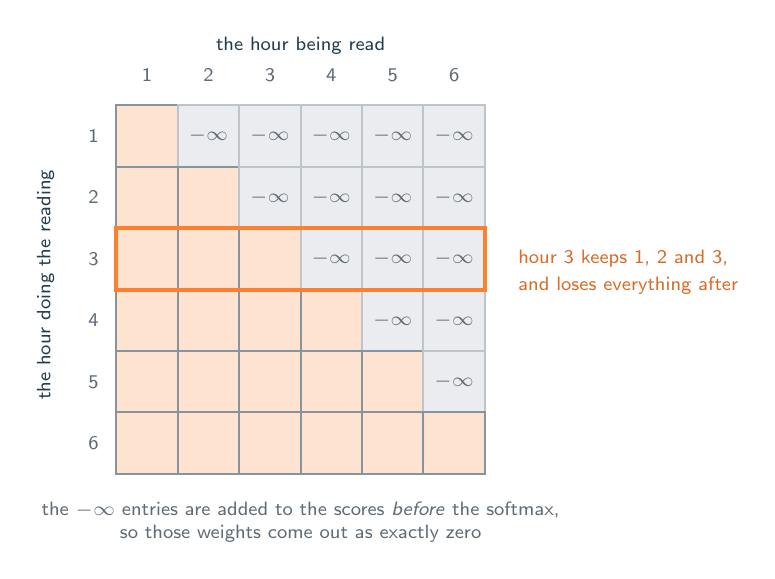
\begin{tikzpicture}[
    every node/.style={font=\sffamily},
    lab/.style={font=\sffamily\scriptsize, text=labelcolor},
    tag/.style={font=\sffamily\scriptsize, text=c2},
    hot/.style={font=\sffamily\scriptsize, text=c3!85!black},
]

\def\cs{0.78}

% column headers: the hour being read
\node[tag] at (3.54, 6.10) {the hour being read};
\foreach \j in {1,...,6}{
    \node[lab] at ({1.20 + (\j-0.5)*\cs}, 5.72) {\j};
}

% row headers: the hour doing the reading
\node[tag, rotate=90] at (0.30, 3.06) {the hour doing the reading};
\foreach \i in {1,...,6}{
    \node[lab, anchor=east] at (1.10, {5.34 - (\i-0.5)*\cs}) {\i};
}

% the grid
\foreach \i in {1,...,6}{
    \foreach \j in {1,...,6}{
        \pgfmathparse{\j<=\i ? 1 : 0}
        \ifnum\pgfmathresult=1
            \filldraw[draw=c2!55, fill=c3!22, line width=0.7pt]
                ({1.20 + (\j-1)*\cs}, {5.34 - \i*\cs})
                rectangle ({1.20 + \j*\cs}, {5.34 - (\i-1)*\cs});
        \else
            \filldraw[draw=c2!30, fill=c4, line width=0.7pt]
                ({1.20 + (\j-1)*\cs}, {5.34 - \i*\cs})
                rectangle ({1.20 + \j*\cs}, {5.34 - (\i-1)*\cs});
            \node[lab] at ({1.20 + (\j-0.5)*\cs}, {5.34 - (\i-0.5)*\cs})
                {$-\infty$};
        \fi
    }
}

% the row we have been following
\draw[c3, line width=1.4pt]
    (1.20, {5.34 - 3*\cs}) rectangle ({1.20 + 6*\cs}, {5.34 - 2*\cs});
\node[hot, anchor=west] at ({1.20 + 6*\cs + 0.30}, {5.34 - 2.5*\cs})
    {hour 3 keeps 1, 2 and 3,};
\node[hot, anchor=west] at ({1.20 + 6*\cs + 0.30}, {5.34 - 2.5*\cs - 0.34})
    {and loses everything after};

\node[lab, anchor=north, align=center] at (3.54, 0.42)
    {the $-\infty$ entries are added to the scores \emph{before} the softmax,\\
     so those weights come out as exactly zero};

\end{tikzpicture}
\end{document}
